\documentclass{article}
\usepackage{graphicx} % new way of doing eps files
\usepackage{listings} % nice code layout
\usepackage[usenames]{color} % color
\definecolor{listinggray}{gray}{0.9}
\definecolor{graphgray}{gray}{0.7}
\definecolor{ans}{rgb}{1,0,0}
\definecolor{blue}{rgb}{0,0,1}
% \Verilog{title}{label}{file}
\newcommand{\Verilog}[3]{
  \lstset{language=Verilog}
  \lstset{backgroundcolor=\color{listinggray},rulecolor=\color{blue}}
  \lstset{linewidth=\textwidth}
  \lstset{commentstyle=\textit, stringstyle=\upshape,showspaces=false}
  \lstset{frame=tb}
  \lstinputlisting[caption={#1},label={#2}]{#3}
}


\author{Josh Young}
\title{Lab 6}

\begin{document}
\maketitle

\section{Introduction}
In Lab 6, the user is tasked with finishing and testing a regfile for the MIPS machine by creating a test bench and running a simulation. The results of the simulation were observed in order to be sure that the regfile is reading and writing properly. Vivado was used to create the test bench as well as run the simulation for the regfile.

\section{Interface}
The Register file has several inputs, these consist of 2 registers, a write register, write control, data to write, a clock, and a reset. There are only a couple of outputs for the register file though, which is just reading data from the registers.

\section{Design}
The register file is an invaluable part of the decoding stage for a MIPS machine. The register file is used as a channel between the decode and write back stages. It is necessary though to use a buffer with the register file, however that isn't addressed in lab 6.

\section{Implementation}
The code used for creating the regfile can be seen in Listing~\ref{code:regfil} on page~\pageref{code:regfil}.

\Verilog{Verilog code for implementing a regfile.}{code:regfil}{../code/2_decode/regfile.v}

\section{Test Bench Design}
The lab had the user create a test bench for the regfile. The goal for the test bench was to try and 'break' the code for the regfile. This test was done by setting the addresses for register A and B, and then changing the writing address as well as the data. Then, the outputs were monitored to be sure that the regfile behaved correctly. The verilog code for the regfile test bench can be viewed in Listing~\ref{code:regtest} on page~\pageref{code:regtest}. 

\Verilog{Verilog code for testing the regfile.}{code:regtest}{../code/2_decode/regfile.v}

\section{Simulation}
By viewing the timing diagrams for the register file test, one can see that the register file behaved as expected. The timing diagram for the register file can be viewed in Figure~\ref{fig:test}. 



\section{Conclusions}
The goal for lab 6 was to finish the register file and create a test bench for it. The simulation shows that the register file acted as it should have. The register file should be able to read from registers and write to registers based off of a given control command.

\begin{figure}
	\begin{center}
		\caption{Timing diagram for the control test.}\label{fig:control_test}
		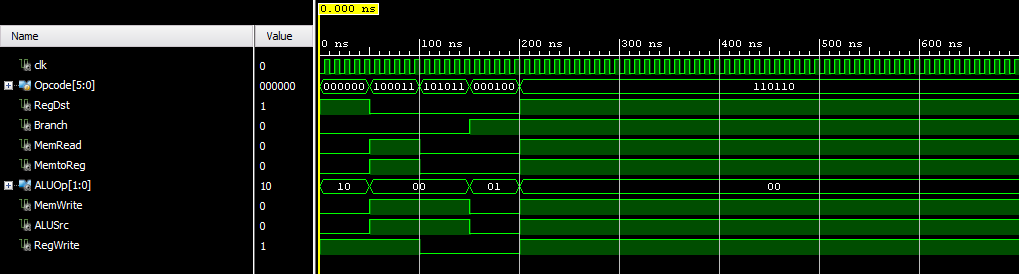
\includegraphics[width=0.9\textwidth]{../images/control_test.png}
	\end{center}
\end{figure}
\begin{figure}
	\begin{center}
		\caption{Timing diagram for the sign extender test.}\label{fig:sign_extend_test}
		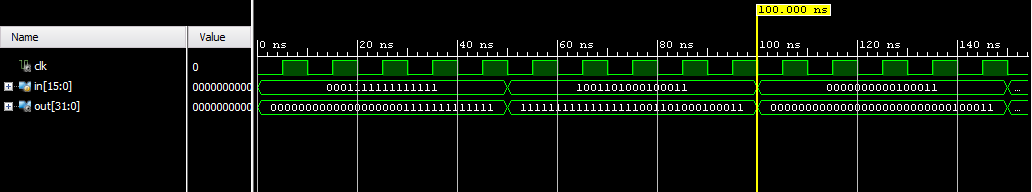
\includegraphics[width=0.9\textwidth]{../images/sign_extend_test.png}
	\end{center}
\end{figure}
\end{document} 
